\part{Manifolds and tensors}

\chapter{Manifolds}

    In physics, we often find problems which involve quantities and operations on them defined in a continuous space: flat spaces, like in classical mechanics and special relativity, or curved spaces, like in general relativity. In this chapter, we will study how we can mathematically describe this kind of spaces through the notion of differentiable manifold.

\section{Differentiable Manifolds}

    A differentiable manifold $\mathcal M$ is a topological space which locally looks like $\mathbb R^n$, but it might have a different and more complicated global topology. This means that if you zoom into a local region, it behaves like a flat $\mathbb R^n$, but over an extended region, you could find a curved region.

\subsection{Topological spaces}

    \begin{definition}[Topological space]
        A topological space $(\mathcal M, \{A_i\})$ is a set of points $\mathcal M$ in which it is defined a topology, i.e.~a family of open sets $\{A_i\}$ such that 
    \begin{enumerate}
        \item the empty set and the whole set are open sets, i.e.
            \begin{equation*}
                \mathcal M, \emptyset \in \{A_i\} ~,
            \end{equation*}
        \item the intersection of a finite number of open sets is an open sets, i.e.
            \begin{equation*}
                \bigcap_{i<\infty} U_i \in \{A_i\} ~,
            \end{equation*}
        \item the union of an arbitrary number of open sets is an open sets, i.e.
            \begin{equation*}
                \bigcap_{i} U_i \in \{A_i\} ~.
            \end{equation*}
    \end{enumerate}
    \end{definition}
    \begin{definition}[Hausdorff space]
    An Hausdorff space is a topological space which has the additional property  
    \begin{equation*}
        \forall P, Q \in \mathcal M \quad \exists U \ni P, V \ni Q \quad \colon \quad U \cap V = \emptyset ~.
    \end{equation*}
    \end{definition}
    \noindent In a topological space, the notions of contiguity and continuity are well defined. Two points are contiguous if they belong to the same open set, called neighbourhood. Intuitively, it means that one is next to the other. A map is an application $\phi \colon D \subset \mathcal M \rightarrow \mathbb R^n$. It is continuous if it maps open sets into open sets. 

\subsection{Charts and atlases}

    \begin{definition}[Chart]
        A chart is a pair $(A, ~\phi)$, where $A \subseteq \mathcal M$ is an open set of a point $P \in \mathcal M$ and $\phi$ is an invertible and continuous map $\phi \colon A \rightarrow \mathbb R^n$, which associates a set of $n$ real coordinates $\phi = x^i$ for the neighbourhood of $P$. See Figure~\ref{fig:chart}
    \end{definition}

    \begin{figure}[h!]
        \centering
        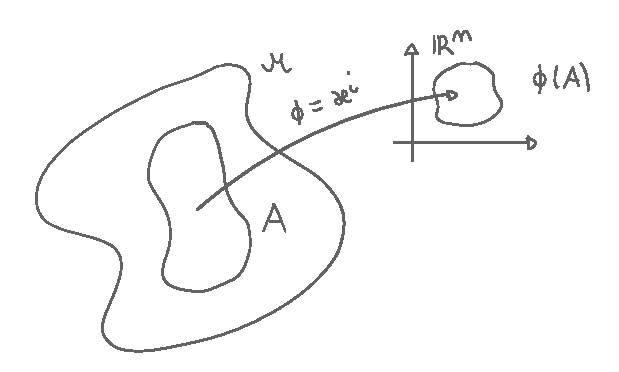
\includegraphics{chart.pdf}
        \caption{A chart on a manifold}\label{fig:chart}
    \end{figure}

    \begin{definition}[Atlas]
        An atlas $\mathcal A$ is a collection of charts that covers entirely the manifold, i.e. 
    \begin{equation*}
        \mathcal A = \{\{(A_i, \phi_i)\} \colon \cup_i A_i \supseteq \mathcal M \} ~.
    \end{equation*}
    \end{definition}
    \noindent In order to include all the points of the manifold $\mathcal M$, neighbourhoods might overlap each others. In the intersection of them, which is open, there are two different coordinate systems that describe the same points and there must be a smooth relation between them. Therefore, an atlas must be endowed with a consistency map.
    \begin{definition}[Consistency map]
        A consistency map between two charts $\phi_1$ and $\phi_2$, over a point $P \in A_1 \cap A_2$, is an invertible map 
        \begin{equation*}
            \psi \colon \phi(A_1) \subseteq \mathbb R^n \rightarrow \phi(A_2) \subseteq \mathbb R^n ~,
        \end{equation*}
        such that 
        \begin{equation*}
            \psi(\phi_1(P)) = \phi_2(P) \quad \textnormal{or} \quad (\phi_2^{-1} \circ \psi \circ \phi_1) = \mathbb I ~,
        \end{equation*}
        or, equivalently, 
        \begin{equation*}
            \psi^{-1} (\phi_2(P)) = \phi_1(P) \quad \textnormal{or} \quad (\phi_1^{-1} \circ \psi \circ \phi_2) = \mathbb I ~.
        \end{equation*}
        See Figure~\ref{fig:consistency}.
    \end{definition}

    \begin{figure}[h!]
        \centering
        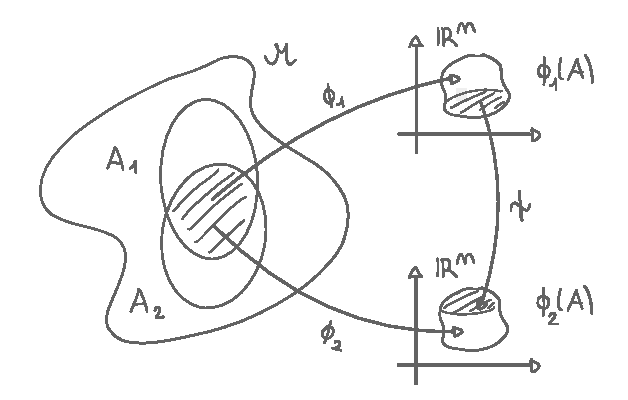
\includegraphics{consistencymap.pdf}
        \caption{A consistency map between two charts on a manifold}\label{fig:consistency}
    \end{figure}

    \noindent Intuitively, a chart is a system of coordinates and an atlas is a system of charts which are smoothly related where they overlapped each others. The consistency map $\psi$ can be seen as a change of coordinates in $\mathbb R^n$. Moreover, since it is invertible, it follows that the dimension $n$ must be the same for all charts and it can be defined as the dimension of the manifold. If $\psi \in C^p(\mathbb R^n)$, then the manifold is a $p$-differentiable manifold. 

\subsection{Manifolds}

    \begin{definition}[Manifold]
        A manifold is an equivalence class of atlases, where two atlases are equivalent if there exists a bijective correspondence between them.
    \end{definition}
    \noindent Examples of manifolds are the $n$-dimensional Euclidean space $\mathbb R^n$, the $n$-dimensional sphere $S^n$, the $n$-dimensional torus $T^n$ or the direct product of two manifolds. Physically related manifolds are the lagrangian configuration space, the hamiltonian phase space or the set of continuous transformations in $\mathbb R^n$. An example of a non-manifold is the cone.

\subsection{Map between manifolds}

    \begin{definition}[Homeomorphism]
        An homeomorphism between two manifold $\mathcal M$ and $\mathcal N$ is an injective, surjective and continuous, with also inverse continuous, map between them. Two manifolds are homeomorphic if it exists such map.
    \end{definition}
    \begin{definition}[Diffeomorphism]
        A diffeomorphism between two manifold $\mathcal M$ and $\mathcal N$ is a smooth (differentiable) homeomorphism. Two manifolds are diffeomorphic if it exists such map.
    \end{definition}
    \noindent Since locally all manifolds of the same dimension $n$ look like $\mathbb R^n$, they can be divide up into classes given by their global properties: two manifolds which are diffeomorphic, and hence they have the same dimension, can be deformed one into each other. 
 
\chapter{Tensors}

\section{Vectors}

    All the objects we will define in this chapter are coordinate-independent. However, for computations purpose, we need to choose them.

\subsection{Curves}

    \begin{definition}[Curve]
        A curve is a continuous map $\gamma \colon I \subseteq \mathbb R \rightarrow \mathcal M$, where $I$ is an open set of $\mathbb R$. The set of all the image points of the function is the ordinary notion of curve. See Figure~\ref{fig:curve}.
    \end{definition} 

    \begin{figure}[h!]
        \centering
        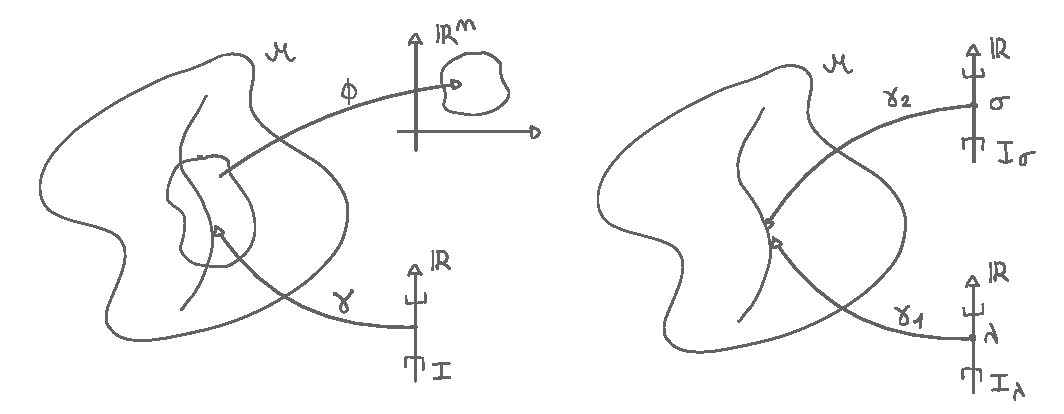
\includegraphics{curve.pdf}
        \caption{A curve on a manifold}\label{fig:curve}
    \end{figure}

    \noindent Given a chart $\phi = x^i$, we can parametrize the curve with a real parameter $\lambda$ and the curve becomes $\phi \circ \gamma \colon I \subseteq \mathbb R \rightarrow \mathbb R^n$, or $x^i = x^i(\lambda)$. If $x^i(\lambda) \in C^p(\mathbb R)$, then $\gamma$ is p-differentiable. A reparameterization $\sigma = \sigma(\lambda)$ defines a different curve, even if the images of the curves coincide.

\subsection{Scalars}

    \begin{definition}
        A function is a map $f \colon \mathcal M \rightarrow \mathbb R$. See Figure~\ref{fig:scalar}.
    \end{definition} 
    \noindent Given a chart $\phi = x^i$, the function becomes $f \circ \phi^{-1} \colon \mathbb R^n \rightarrow \mathbb R$, or $f = f(x^i)$. Given another chart $\phi' = y^j$, $f'(y(P)) = f(x(P))$, showing that it is indeed a scalar. If $f(x^i) \in C^p(\mathbb R)$, then $f$ is $p$-differentiable. The coordinates are themselves $\infty$-differentiable functions.

    \begin{figure}[h!]
        \centering
        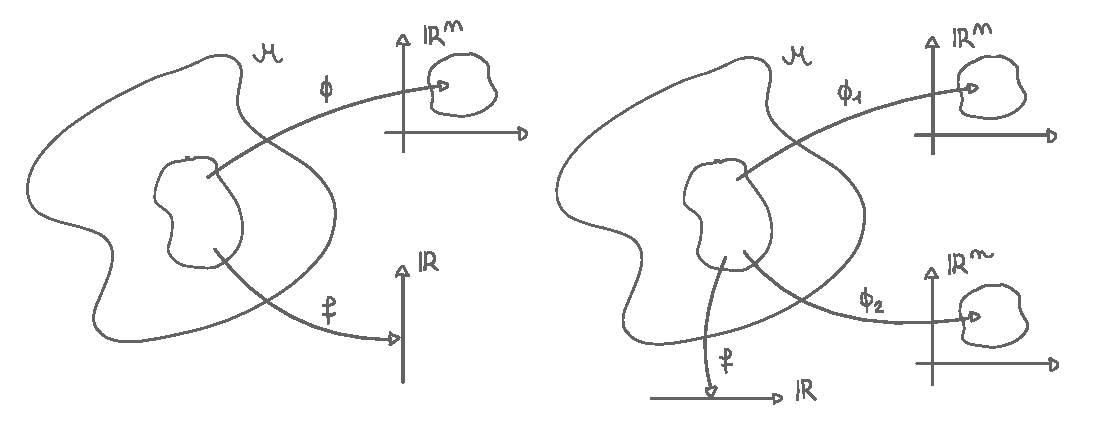
\includegraphics{scalar.pdf}
        \caption{A scalar on a manifold}\label{fig:scalar}
    \end{figure}

\subsection{Vectors}

    Given that we have not defined a notion of distance, vectors are not anymore displacements or arrows between two points, but tangent objects to a curve defined at a single point.

    \begin{definition}[Vector]
        A vector at a point $P \in \mathcal M$ is a functional map that associates to a function its derivative $v_{\gamma, P} \colon f \rightarrow v_\gamma(f) = \dv{f}{\lambda} \Big \vert_{\lambda_P} \in \mathbb R$, where $\gamma(\lambda_P) = P$.
    \end{definition} 
    \noindent Given a chart $\phi = x^i$,
    \begin{equation*}
    \begin{aligned}
        v_{\gamma P} (f) & = \dv{(f \circ \gamma)}{\lambda} \Big\vert_{\lambda_P} \\ & = \dv{}{\lambda} (f \circ \mathbb I \circ \gamma) \Big\vert_{\lambda_P} \\ & = \dv{}{\lambda} (f \circ \phi^{-1} \circ \phi \circ \gamma) \Big\vert_{\lambda_P} \\ & = \dv{}{\lambda} (f(x^i) \circ x^i(\lambda)) \Big\vert_{\lambda_P} \\ & = \dv{}{\lambda} f(x^i(\lambda)) \Big\vert_{\lambda_P} = \pdv{f}{x^i} \dv{x^i}{\lambda}
    \end{aligned}
    \end{equation*}
    and since it is true $\forall f$
    \begin{equation*}
        v_\gamma = \dv{}{\lambda} = \dv{x^i}{\lambda} \pdv{}{x^i} 
    \end{equation*}
    which means that a vector is the tangent to a curve $\gamma$ at a point $P$. We can interpret those terms as
    \begin{equation*}
        v = \underbrace{\dv{x^i}{\lambda}}_{v_i} \underbrace{\pdv{}{x^i}}_{e_i} = v^i e_i
    \end{equation*}
    where $v^i$ are the components and $e_i$ are the coordinate basis vectors. 
    
    \begin{definition}[Coordinate basis vectors]
        Coordinate basis vectors are those vectors which are tangent to the coordinate line defined by constant $x^j$ for $i \neq j$.
    \end{definition}

    Since any curve has an unique parameter, it has also a unique tangent vector. Conversely, a vector is tangent to an infinite number of curves, because there are different curves with the same tangent vector or the same curve can be reparameterised to give rise to another tangent vector.

    Under a change of coordinates $y^i = y^i(x^j)$, the components transform by 
    \begin{equation*}
        v^i = \dv{x^i}{\lambda} = \pdv{x^i}{y^{j'}} \dv{y^{j'}}{\lambda} = \pdv{x^i}{y^{j'}} v^{j'}
    \end{equation*}
    and the basis vectors transform by 
    \begin{equation*}
        e_i = \pdv{}{x^i} = \pdv{y^{j'}}{x^i} \pdv{}{y^{j'}} = \pdv{y^{j'}}{x^i} e_{j'}
    \end{equation*}
    \noindent Notice that components transform but basis change too, inversely, and, as a consequence, the vector remains the same, which shows that it is coordinate-independent.

    \begin{definition}
        A vector field in an open set $U \subseteq \mathcal M$ is map from each point $P \in U$ into a vector $v(P)$.
    \end{definition} 
    \noindent Given a chart $\phi = x^i$, the vector field becomes $v (x^i) = v \circ \phi^{-1}$. Intuitively, it is a rule that associates a vector for each point. The components of a vector field depend on coordinates $V = v^i(x^j) e_i$.

    By definition a vector is a linear functional
    \begin{equation*}
        v_\gamma (af + bg) = \dv{}{\lambda} (af+bg) = a \dv{f}{\lambda} + b \dv{g}{\lambda}
    \end{equation*}

    The coordinate vectors $e_i = \pdv{}{x^i}$ form a basis of a linear space composed by all the vectors tangent to a point $P$, called the tangent space $T_P$.

    \begin{proof}
    Firstly, every tangent vector can be expressed as linear combination. Infact, consider two curves, parametrized by $\lambda$ and $\sigma$, across a point $P$ which generate two vectors $v = \pdv{}{\lambda}$ and $w = \dv{}{\sigma}$. Hence, a generic linear combination of them is vector as well
    \begin{equation*}
        a v + b w = a \dv{}{\lambda} + b \dv{}{\sigma} = a \pdv{x^i}{\lambda} \pdv{}{x^i} + b \dv{x^i}{\sigma} \pdv{}{x^i} = \Big ( a \pdv{x^i}{\lambda} + b \dv{x^i}{\sigma} \Big ) \pdv{}{x^i} = \Big ( a \pdv{x^i}{\lambda} + b \dv{x^i}{\sigma} \Big ) e_i
    \end{equation*}
    Since there are $n$ coordinates $x^i$, we have $n$ indipendent curves.

    Secondly, the coordinate basis vectors are linearly independent. 
    Infact, by the inverse function theorem which says that a map is $1-1$ if and only if the determinant of the jacobian matrix of $y^i = y^i(x^j)$ is not vanishing
    \begin{equation*}
        \det J = \det 
        \begin{pmatrix}
            \pdv{y^1}{x^1} & \cdots & \pdv{y^1}{x^n} \\
            \cdots & \cdots & \cdots \\
            \pdv{y^n}{x^1} & \cdots & \pdv{y^n}{x^n} \\
        \end{pmatrix} \neq 0
    \end{equation*}
    Hence, there are $n$ columns (or rows) which are linearly independent and also $n$ basis vector
    \begin{equation*}
        e_i = \pdv{}{x^i} = \pdv{y^j}{x^i} \pdv{}{y^j}
    \end{equation*}
    \end{proof}

    The dimension of $T_P$ is the same as the manifold. In other words, there is a $1-1$ correspondence between $T_P$ and the space of all derivative along curves in $P$. 

    It is important to remark that coordinate basis vectors at different points belong to different tangent space and cannot be linearly combined.

\subsection{Fiber bundles}

    A tangent bundle is the set of all tangent space at each point together with the manifold itself $\mathcal T \mathcal M = \{\mathcal M, ~\{T_P \colon \forall P \in \mathcal M \}\}$. It can be shown that $\mathcal T \mathcal M$ is a manifold too. The dimension of the tangent bundle is $2n$. 

\subsection{Exponential maps}

    So far, we have defined a tangent vector given a curve, but now we want to examine the inverse problem. 
    
    \begin{definition}[Integral curve]
        An integral curve $\gamma = \gamma(\lambda)$ of a vector field $V$ is the curve which as tangent vector $\dv{}{\lambda}$ has the element of $V$ in $P \in \gamma$, i.e. 
        \begin{equation*}
            V = \dv{}{\lambda}
        \end{equation*}
    \end{definition}

    Given a chart $\phi = x^i$ and a point $P_0$,
    \begin{equation} \label{cauchy}
        \begin{split}
            V^i(\lambda) = \dv{x^i(\lambda)}{\lambda} \\
            x^i(P_0) = x^i(\lambda_0)
        \end{split}
    \end{equation}
    which are a system of $n$ Cauchy problems, first-order ordinary differential equations with initial conditions, and the components of $V$ at an arbitrary point $P = \phi^{-1}(x^i(\lambda))$ are $V(P) = V^i(x^j(\lambda)) \pdv{}{x^i} = V^i(\lambda) \pdv{}{x^i}$. Theorems of calculus in $\mathbb R^n$ ensure that locally tha solution of~\eqref{cauchy} always exists, which is indeed the integral curve $\gamma(\lambda)$. Integral curves can never cross each other (except possibly at $V = 0$). 

    Formally, the solution of~\eqref{cauchy} is the exponential map
    \begin{equation*}
        x^i(\lambda) = \exp((\lambda - \lambda_0)V) x^i \Big\vert_{\lambda_0}
    \end{equation*}
    which describes the flow of $V$ in a neighbourhood of $P$. 

    \begin{proof}
        Let $V = \dv{}{\lambda}$ be a vector fields with integral curve $\gamma = \gamma (\lambda)$. Given a chart $x^i$, we can Taylor expand around $P_0$ along $\gamma$
        \begin{equation*}
        \begin{aligned}
            x^i(\lambda_0 + \epsilon) & = x^i(\lambda_0) + \epsilon \dv{x^i}{\lambda} \Big\vert_{\lambda_0} + \frac{\epsilon^2}{2} \dvd{x^i}{\lambda} \Big\vert_{\lambda_0} + \ldots \\ & = \Big (1 + \epsilon \dv{}{\lambda} \Big\vert_{\lambda_0} + \frac{\epsilon^2}{2} \dvd{}{\lambda} \Big\vert_{\lambda_0} + \ldots \Big) ~ x^i(\lambda_0) \\ & = \exp(\epsilon \dv{}{\lambda}) ~ x^i \Big\vert_{\lambda_0} \\ & = \exp(\epsilon V) ~ x^i \Big\vert_{\lambda_0} 
        \end{aligned}
        \end{equation*}
    \end{proof}
    \noindent Since $\epsilon \dv{}{\lambda}$ is an infinitesimal motion, the exponential map allows to move in a finite way.
    
    For an arbitrary function $f$ in a neighbourhood of $P$
    \begin{equation*}
        f(\lambda_0 + \epsilon) = \exp \Big(\epsilon \dv{}{\lambda} \Big) ~ f \Big\vert_{\lambda_0} = \exp (\epsilon V ) ~ f \Big\vert_{\lambda_0}
    \end{equation*}

\subsection{Lie brackets}

    Any linearly independent set of vector fields can be used as basis, but not all of them are coordinate vector basis. 

    \begin{definition}
        The Lie brackets, or the commutator, of two vector fields $V = \dv{}{\lambda}$ and $W=\dv{}{\mu}$ are 
        \begin{equation*}
            [V, W] = \dv{}{\lambda} \dv{}{\mu} - \dv{}{\mu} \dv{}{\lambda}
        \end{equation*}
    \end{definition}

    Given a chart $\phi = x^i$, the Lie brackets become
    \begin{equation*}
    \begin{aligned}
        [V, ~W] & = \dv{}{\lambda} \dv{}{\mu} - \dv{}{\mu} \dv{}{\lambda} \\ & = v^i \pdv{}{x^i} \Big( w^j \pdv{}{x^j} \Big) - w^i \pdv{}{x^i} \Big( v^j \pdv{}{x^j} \Big) \\ & = \cancel{v^i w^j \pdv{}{x^i} \pdv{}{x^j}} + v^i \pdv{w^j}{x^i} \pdv{}{x^j} - \cancel{v^j w^i \pdv{}{x^i} \pdv{}{x^j}} - w^i \pdv{v^j}{x^i} \pdv{}{x^j} \\ & = \Big ( v^i \pdv{w^j}{x^i} - w^i \pdv{v^j}{x^i} \Big ) \pdv{}{x^j} 
    \end{aligned}
    \end{equation*}
    where it is used the facf that the partial derivatives commute. Hence the commutator of two vectors is still a vector. 

    The geometrical meaning of the commutator is the following: consider two vector fields $V = \dv{}{\lambda}$ and $W = \dv{}{\mu}$. According with the exponential map, the coordinates of A, moving before along $V$ and then along $W$, are 
    \begin{equation*}
        x^i(A) = \exp \Big ( \epsilon_2 \dv{}{\mu} \Big) \exp \Big ( \epsilon_1 \dv{}{\lambda} \Big) ~ x^i \Big\vert_P
    \end{equation*}
    while the coordinates of B, moving before along $W$ and then along $Y$, are 
    \begin{equation*}
        x^i(B) = \exp \Big ( \epsilon_1 \dv{}{\lambda} \Big) \exp \Big ( \epsilon_2 \dv{}{\mu} \Big) ~ x^i \Big\vert_P
    \end{equation*}
    Computing the difference
    \begin{equation*}
        x^i(B) - x^i(A) = \epsilon_1 \epsilon_2 \Big [\dv{}{\lambda}, ~\dv{}{\mu} \Big ] ~ x^i \Big\vert_P + O(\epsilon^3)
    \end{equation*}
    Hence, if the commutator does not vanish, the final points are different $A \neq B$ and the path $PA \cup PB$ does not close. 

    A sufficient and necessary condition for a set of fields to be coordinate vectors is that their commutator vanishes. 
    \begin{proof}
    Firstly, the necessary condition. Consider two coordinate vector fields $V = \pdv{}{x^1}$ and $W = \pdv{}{x^2}$. Then $v^i = \pdv{x^i}{x^1} = \delta^i_{\phantom i 1}$, $w^j = \pdv{x^j}{x^2} = \delta^j_{\phantom j 2}$ and the commutator vanishes, since the derivative of a constant is null. 

    Secondly, the sufficient condition. Consider two commuting vector fields $V = \pdv{}{x^1}$ and $W = \pdv{}{x^2}$. Suppose also that they are linearly independent
    \begin{equation} \label{proof2}
        a V(P) + b W(P) = 0 \quad \iff \quad a = b = 0.
    \end{equation}
    Given a chart $\phi = x^i$, according with the exponential map, the motion from $P$ along $V$ by $\Delta \lambda = \alpha$ to a point $R$ is
    \begin{equation*}
        x^(R) = \exp \Big (\alpha \dv{}{\lambda} \Big) ~ x^i \Big\vert_P
    \end{equation*}
    and then along $W$ by $\Delta \mu = \beta$ to a point $Q$ is
    \begin{equation}\label{proof1}
        x^(Q) = \exp \Big (\beta \dv{}{\mu} \Big) \exp \Big (\alpha \dv{}{\lambda} \Big) ~ x^i \Big\vert_P
    \end{equation}
    If $\alpha$ and $\beta$ are coordinates, the corresponding components of the basis vectors are $\pdv{x^i}{\alpha}$ and $\pdv{x^i}{\beta}$.
    Hence, using~\eqref{proof1}
    \begin{equation*}
    \begin{aligned}
        \pdv{x^i}{\alpha} & = \pdv{}{\alpha} \Big ( \exp \Big( \beta \dv{}{\mu} \Big) \exp \Big( \alpha \dv{}{\lambda} \Big) ~ x^i \Big\vert_P \Big) \\ & = \exp \Big( \beta \dv{}{\mu} \Big) \pdv{}{\alpha} \Big ( \exp \Big( \alpha \dv{}{\lambda} \Big) ~ x^i \Big\vert_P \Big) \\ & = \exp \Big( \beta \dv{}{\mu} \Big) \exp \Big( \alpha \dv{}{\lambda} \Big) ~ \dv{x^i}{\lambda} \Big\vert_P
    \end{aligned}
    \end{equation*}
    and, similarly, 
    \begin{equation*}
        \pdv{x^i}{\beta} = \exp \Big( \beta \dv{}{\mu} \Big) \exp \Big( \alpha \dv{}{\lambda} \Big) ~ \dv{x^i}{\mu} \Big\vert_P
    \end{equation*}
    This shows that $\pdv{}{\alpha}$ and $\pdv{}{\beta}$ are respectively the vector fields $\dv{}{\lambda}$ and $\pdv{}{\mu}$ evaluated in $Q$, using the fact that the commutator is vanishing. 
    \begin{equation*}
        \pdv{}{\alpha} = \dv{}{\lambda} \quad \pdv{}{\beta} = \dv{}{\mu}
    \end{equation*}
    Finally, the determinant of the Jacobians is not zero
    \begin{equation*}
        \det J = \det \begin{bmatrix}
            \pdv{x^1}{\alpha} & \pdv{x^2}{\alpha} \\
            \pdv{x^1}{\beta} & \pdv{x^2}{\beta} \\
        \end{bmatrix} \neq 0
    \end{equation*}
    since we assumed the linearly independence of $\dv{}{\lambda}$ and $\dv{}{\mu}$. In this way we built a $1-1$ map which provides a coordinate system.

    The proof can be extended to $n$ dimensions: $n$ linearly dependent commuting vector fields $V_i$ are a coordinate basis $\alpha_i$ in which an arbitrary element can be written as 
    \begin{equation*}
        x^j(\alpha_i) = \exp (\sum_i \alpha_i V_i) x_j \vert_P
    \end{equation*}
    \end{proof} 

    In non-coordinate basis, vector fields cannot be expressible in terms of partial derivatives of coordinates. Hence, an integral curve of $V$ is not necessarily a curve of constant $\mu$ and viceversa. For instance, $x^i$ are the integral curves of $\pdv{}{x^i}$ and $x^j$ with $j\neq i$ are constant along those curves, all because they are coordinate basis. It is important to notice that the difference between coordinate and non-coordinate bases can be sees only in a region of the manifold. Thus, in a point there is no different because they are both basis of $T_P$. Intuitively, a coordinate basis can be represented as a grid in which all lines intersect each others.

\section{1-forms}

    \begin{definition}[1-form]
        A 1-form is a linear functional $\omega$ acting on a vector $\omega \colon T_P \rightarrow \mathbb R$ such that $\omega(\alpha v + \beta u) = \alpha \omega(v) + \beta \omega(u)$ and $(\alpha \omega + \alpha \sigma)(v) = \alpha \omega(v) + \beta \sigma(v)$. 
    \end{definition}
    Linearity implies that the action of a 1-form is completely determined by the action on a basis of $T_P$. 1-forms acting on the same $T_P$ form a linear space $T^*_P$, called the cotangent space. A cotangent bundle is the set of all cotangent space at each point together with the manifold itself $\mathcal T^* \mathcal M = \{\mathcal M, ~\{T^*_P \colon \forall P \in \mathcal M \}\}$. A 1-form field is a map which associates a 1-form of $T^*P$ to each point $P \in \mathcal M$. 

    Examples of 1-forms are row vectors in linear algebra and bras in quantum mechanics.

    One way of thinking 1-forms is in the following way: given an arbitrary function, a vector field is defined by $V(f) = \dv{f}{\lambda}$ whereas given an arbitrary vector field, a 1-form is defined by $V(f) = \dv{f}{\lambda} = df (\dv{}{\lambda})$. The difference is the in the former $V$ is fixed and $f$ is arbitrary, whereas in the latter $f$ is fixed and $V$ is arbitrary. Given a chart $\phi = x^i$
    \begin{equation*}
        \dv{f}{\lambda} = \pdv{f}{x^i} \dv{x^i}{\lambda} = \nabla_i f \dv{x^i}{\lambda} = df_i \dv{x^i}{\lambda}
    \end{equation*}
    where $df_i$ are the components of the 1-form $df$, called the gradient of $f$.
    
    Geometrically, the gradient of a function can be seen as the number of contour lines that a vector $V$ crosses in a neighbourhood of $P$. Generalizing for 1-forms, they can be seen as a set of level surfaces whose action on a vector is the number of surface the vector crosses. Generalizing, a 1-form may be seen as a series of surface and its action on a vector is the number of surfaces that the vector crosses. The closer the surfaces, the larger the 1-form.

    Let $\{e_i\}$ be a basis of $T_P$. A basis of $T^*_P$ is not related to it. Any $n$ linearly independent 1-forms constitue a basis. However it is convenient to choose the dual basis, which completely defined a basis of $T^*P$ by a basis in $T_P$ in the following way
    \begin{equation}\label{dual}
        e^i(e_j) = \delta^i_{\phantom i j}
    \end{equation}
    or, equivalently, applying it to a vector $v$
    \begin{equation*}
        e^i(V) = e^i(V^j e_j) = V^j e^i(e_j) = V^j \delta^i_{\phantom i j} = V^i
    \end{equation*}
    A change in one of the basis vector generally changes all the basis 1-forms.

    Consequently, $\mathcal M$, $T_P$ and $T^*_P$ have the same dimension $n$. $\{e^i\}$ are actually a basis of $T^*_P$, since given an arbitrary 1-form $q$
    \begin{equation*}
        q(v) = q(v^i e_i) = v^i q(e_i) = v^i q_i
    \end{equation*}
    and
    \begin{equation*}
        v^i q_i = q_i e^i(v)
    \end{equation*}

    Remember that under a change of coordinates, vectors or 1-forms do not change, only their components and basis change, the latter inversely.

    A coordinate system defines automatically a set of 1-forms $dx^i$ such that $dx^i (\pdv{}{x^j}) = \pdv{x^i}{x^j} = \delta^i_{\phantom i j}$. Hence differentials are the basis 1-form dual to the coordinate basis vectors 
    \begin{equation*}
        \dv{f}{\lambda} = \pdv{f}{x^i} \dv{x^i}{\lambda} = \pdv{f}{x^i} dx^i \Big(\dv{x^j}{\lambda} \pdv{}{x^j} \Big) = \pdv{f}{x^i} \dv{x^j}{\lambda} dx^i \Big ( \pdv{}{x^j} \Big) = \pdv{f}{x^i} \pdv{x^j}{\lambda} \delta^i_{\phantom i j} = \pdv{f}{x^i} \pdv{x^i}{\lambda}
    \end{equation*}    

\section{Tensors}  

    \begin{definition}[Tensor]
        A tensor $(n, m)$ at $P$ is a multi-linear, i.e.~linear on every argument, functional that maps $n$ 1-forms and $m$ vectors into a real number 
        \begin{equation*}
            T \colon \underbrace{T^*_P \otimes \cdots \otimes T^*_P}_{n~times} \otimes \underbrace{T_P \otimes \cdots \otimes T_P}_{m~times} \rightarrow \mathbb R
        \end{equation*}
    \end{definition}

    A tensor can be also seen as the outer product of 1-forms and vectors. A tensor $(1, 0)$ is a vector, a tensor $(0, 1)$ is a 1-form, a tensor $(0,0)$ is a scalar. A $(1,1)$ tensor is a 1-form if $T(\omega, ~)$, since a vector is mapped into a real number, and a vector if $T(~, V)$, since a 1-form is mapped into a real number.
    
    A tensor $(n, m)$ can be written in terms of the vector basis and its dual one
    \begin{equation*}
        T = T^{i_1 \cdots i_n}_{j_1 \cdots j_m} e_{i_1} \otimes \cdots \otimes e_{i_n} \otimes e^{j_1} \otimes \cdots \otimes e^{j_m}
    \end{equation*}
    where the components are the values when basis are taken
    \begin{equation*}
        T^{i_1 \cdots i_n}_{j_1 \cdots j_m} = T(e^{i_1}, ~\cdots, ~e^{i_n}, ~e_{j_1}, ~\cdots, ~e^{j_m})
    \end{equation*}

    A change of basis is determined by a $4 \times 4$ non-degenerate matrix $\Lambda \in GL(n)$. On a vector basis, it acts as 
    \begin{equation}\label{proof4}
        {e'}_j = \Lambda^i_{\phantom i j} e_i
    \end{equation}
    This transformation has no effects on the dual space. However, in order to keep the duality of the basis, it must induce a transformation with the inverse matrix to the dual basis
    \begin{equation*}
        {e'}^j = \Lambda^j_{\phantom j i} e^i
    \end{equation*}

    \begin{proof}
        Recalling~\eqref{dual}, to preserve the duality, also the transformed dual basis must obey 
        \begin{equation}\label{proof3}
            {e'}^i ({e'}_j) = \delta^i_{\phantom i j}
        \end{equation}
        Hence, given an arbitrary transformation matrix, 
        \begin{equation*}
            {e'}^i = M^i_{\phantom i k} e^k
        \end{equation*}
        and putting into~\eqref{proof3}, using\eqref{proof4}
        \begin{equation*}
            \delta^i_{\phantom i j} = {e'}^i ({e'}_j) = M^i_{\phantom i k} e^k (\Lambda^l_{\phantom l j} e_l) = M^i_{\phantom i k} \Lambda^l_{\phantom l j} e^k(e_l) = M^i_{\phantom i k} \Lambda^l_{\phantom l j} \delta^k_{\phantom k l} = M^i_{\phantom i k} \Lambda^k_{\phantom k j}
        \end{equation*}
        then, $M$ must satisfy
        \begin{equation*}
            M^i_{\phantom i k} \Lambda^k_{\phantom k j} = \delta^i_{\phantom j} 
        \end{equation*}
        and it is indeed the inverse matrix.
    \end{proof}

    It is possible to perform several operations on tensors at $P$:
    \begin{enumerate}
        \item scalar multiplication, i.e. 
            \begin{equation*}
                S^{(n,m)} = a T^{(n,m)} \quad \forall a \in \mathbb R
            \end{equation*}
        \item addition, i.e. 
            \begin{equation*}
                S^{(n,m)} = T^{(n,m)} + Q^{(n,m)}
            \end{equation*}
        \item outer product, i.e. 
            \begin{equation*}
                S^{(n+p,m+q)} = T^{(n,m)} \otimes Q^{(p,q)}
            \end{equation*}
        \item saturation with 1-forms, i.e. 
            \begin{equation*}
                T^{(n-1,m)} = T^{(n,m)} (\ldots, ~w, ~\ldots)
            \end{equation*}
        \item saturation with vector, i.e. 
            \begin{equation*}
                T^{(n,m-1)} = T^{(n,m)} (\ldots, ~v, ~\ldots)
            \end{equation*}
    \end{enumerate}
    The last two can be generalised to an arbitrary saturation of a $(n,m)$ tensor with a $(p<n, q<m)$ tensor. 

    For a change of basis in the tangent space to correspond a change of coordinates in a neighbourhood on the manifold, the transformation matrix must obey the condition
    \begin{equation}\label{proof8}
        \pdv{\Lambda^j_{\phantom j i}}{x^k} = \pdv{\Lambda^j_{\phantom j k}}{x^i}
    \end{equation}

    \begin{proof}
        Consider two charts $x^i$ and $y^i$ that overlap at $P$. The transformation matrix between basis is 
        \begin{equation*}
            \Lambda^i_{\phantom i j} = \pdv{x^i}{y^j}
        \end{equation*}
        and the inverse is 
        \begin{equation*}
            \Lambda^j_{\phantom j i} = \pdv{y^j}{x^i}
        \end{equation*}

        If we move continuously to another point $Q$ insider the charts, the matrix transformation will become a field $\Lambda(Q) = \Lambda(x^i(Q)) = \Lambda(y^i(Q))$ and, since the partial derivatives commute
        \begin{equation*}
            \pdv{\Lambda^j_{\phantom j i}}{x^k} = \pdv{}{x^k} pdv{y^j}{x^i} = \pdv{}{x^i} pdv{y^j}{x^k} = \pdv{\Lambda^j_{\phantom j k}}{x^i}
        \end{equation*}
    \end{proof}

    Hence, on a point $P$, the matrix transformation ha $n^2$ degrees of freedom, while in a neighbourhood of $P$, it has less of them. It is another way to say that a vector field basis is not always a coordinate basis.

\chapter{Lie derivatives}

    In order to define a derivative on the manifold, we need to find a way to compare vectors which live in tangent spaces of different points. In this chapter, we will introduce the notion of Lie derivative, which exploits congruences of a vector field to move objects on the manifold.

\section{Active and passive transformation}

    Diffeomorphisms and coordinate change are two different ways to do the same thing. 
    
    A coordinate change is just the introduction of a new coordinate map $y = y(x)$, but the points on the manifold remain fixed. The diffeomorphism does not act on $\mathcal M$, but on the coordinates in $\mathbb R^n$. It can be sees as a change of coordinates $x' = x'(x, \epsilon)$ where $\epsilon$ is a parameter such that $x'(x, 0) = x$. For instance, a function changes in such a way that $\Phi'(x') = \Phi(x)$ where $\Phi(x) = (f \o \phi^{-1})(x)$. It is called a passive intepretation of a diffeomorphism.

    In the active interpretation of a diffeomorphism, the points are actually moved (along the flow of an integral curve). The diffeomorphism do act on $\mathcal M$. 

\section{Congruence}

    A congruence of a vector field $V$ is a set of integral curve which start from a curve an hypersurface $\Sigma_0$ of dimension $n-1$ and uniquely cover a portion of $\mathcal M$, without insersecting. The set of curves has dimension $(n-1)$. This means that in each point $P$ pass one and only one curve. Thus, congruence provides a natural way to move in the manifold. 
    
    \begin{definition}[Push-forward]
        A push-forward, or Lie dragging, $\phi_{\Delta \lambda} \colon \mathcal M \rightarrow \mathcal M$ is the motion of a point $P(\lambda_0)$ in $P(\lambda_0 + \Delta \lambda)$ such that $\phi_{\Delta \lambda}$ is continuous and invertible.
    \end{definition} 
    
    If $V \in C^{\infty}$, the push-forward becomes a diffeomorphism and form a group. Infact, $\phi_{\lambda_1} \o \phi_{\lambda_2} = \phi_{\lambda_1 + \lambda_2}$, $\phi_{\lambda}^{-1} = \phi_{- \lambda}$ and $\phi_{\lambda = 0} = \mathbb I$. 

    \begin{definition}[Push-forward of a function]
        The push-forward of a function $f$ along a congruence of $V = \dv{}{\lambda}$ is a map $f^*$ from a point $P$ to a point $Q = \phi_{\Delta \lambda}(P) $ such that
        \begin{equation*}
            f^*_{\Delta \lambda} (Q) = f(P) 
        \end{equation*}
    \end{definition}
    If it is true $\forall Q$ along the integral curve of $V$, $f^*_{\Delta \lambda}$ is constant and $\dv{f}{\lambda} = 0$.

    \begin{definition}[Push-forward of a vector field]
        The push-forward of a vector field $W = \dv{}{\mu}$ along a congruence of $V = \dv{}{\lambda}$ is a map $f^*$ from a point $P$ to a point $Q = \phi_{\Delta \lambda}(P) $ such that
        \begin{equation*}
            W^*_{\Delta \lambda} (f^*_{\Delta \lambda}) \vert_Q = W (f) \vert_P
        \end{equation*}
        where $f$ is an arbitrary function, or, equivalently written  
        \begin{equation*}
            \dv{f^*}{\mu} \Big\vert_{\lambda_0 + \Delta \lambda} = \dv{f}{\mu}
        \end{equation*}
        where $\lambda(P) = \lambda_0$ and $\lambda(Q) = \lambda_0 + \Delta \lambda$.
    \end{definition}
    
    Furthermore, the commutator between $V$ and $W^*$ vanishes
    \begin{equation}\label{comm}
        [V, W^*] = [\dv{}{\lambda}, \dv{}{\mu^*}] = 0
    \end{equation}

    \begin{proof}
        Fixing $f$ and varying $\Delta \lambda$, $\dv{f^*}{\mu^*}$ is constant along the congruences of $V$. Mapping the initial curve $\Sigma_0$ into a new curve $\Sigma_{\Delta \lambda}$ and since $\lambda$ is constant, it can be used as a coordinate. 

        Since $W^*$ is tangent to $\Sigma_{\Delta \lambda}$ its parameter $\mu^*$ is constant along the congruences of $V$. Hence there are two coordinates $(\lambda, \mu^*)$ are coordinates and their coordinate vectors commute.
    \end{proof}

    Intuitively, the commutator is vanishing, and they form a coordinate basis, because a vector field is dragged only if it is constant along a congruence of the othe vector, which is the definition of coordinate basis.

\section{Lie derivatives}

    The push-forward allows us to move a point from $\lambda + \Delta \lambda$ to $\lambda$ and compare vectors or functions defined in two different point.

    \begin{definition}[Lie derivative of a function]
        The Lie derivative of a function $f$ along a vector field $V=\dv{}{\lambda}$ is 
        \begin{equation} \label{liederf}
            \pounds_{V} f =  V(f)
        \end{equation}
        
    \end{definition} 
    If $f$ is constant along the congruences, then $\pounds_V f = 0$.

    \begin{proof}
        \begin{equation*}
            \pounds_{V} f \vert_{\lambda_0} = \lim_{\Delta \lambda \rightarrow 0} \frac{f^*_{-\Delta \lambda}(\lambda_0) - f(\lambda_0)}{\Delta \lambda} = \lim_{\Delta \lambda \rightarrow 0} \frac{f(\lambda_0 + \Delta \lambda)- f(\lambda_0)}{\Delta \lambda} = \dv{f}{\lambda} \Big \vert_{\lambda_0} = V(f)
        \end{equation*}
        where it has been used the push-back $\phi_{-\Delta\lambda} (P(\lambda_0 + \Delta \lambda)) = P(\lambda_0)$ and $f^*_{-\Delta\lambda} (\lambda_0) = f (\lambda_0 + \Delta \lambda)$.
    \end{proof}

    \begin{definition}[Lie derivative of a vector field]
        The Lie derivative of a vector field $W=\dv{}{\mu}$ along a vector field $V=\dv{}{\lambda}$ is
        \begin{equation}\label{liederfv}
            \pounds_V W = [V, W]
        \end{equation}
    \end{definition}

    \begin{proof}
        \begin{equation*}
            \pounds_V W (f) \vert_{\lambda_0} = \lim_{\Delta \lambda \rightarrow 0} \frac{W^*_{-\Delta\lambda} - W}{\Delta \lambda} (f) \Big \vert_{\lambda_0}
        \end{equation*}
        Taylor expanding around $\lambda_0 + \Delta \lambda$ 
        \begin{equation*}
            W^*_{-\Delta\lambda} (f) \Big \vert_{\lambda_0} = \dv{f}{\mu^*} \Big \vert_{\lambda_0} = \dv{f}{\mu^*} \Big \vert_{\lambda_0 + \Delta \lambda} - \Delta \lambda \Big ( \dv{}{\lambda} \dv{}{\mu^*} f \Big)\Big \vert_{\lambda_0 + \Delta \lambda} + O(\Delta \lambda^2)
        \end{equation*}
        Using~\eqref{comm} and at first order $\dv{}{\mu} = \dv{}{\mu^*}$,
        \begin{equation*}
        \begin{aligned}
            \dv{f}{\mu^*} \Big \vert_{\lambda_0} & = \dv{f}{\mu} \Big \vert_{\lambda_0 + \Delta \lambda} - \Delta \lambda \Big ( \dv{}{\lambda} \dv{}{\mu^*} f \Big)\Big \vert_{\lambda_0 + \Delta \lambda} + O(\Delta \lambda^2) \\ & = \dv{f}{\mu} \Big \vert_{\lambda_0} + \Delta \lambda \dv{}{\lambda} \dv{}{\mu^*} f \Big \vert_{\lambda_0} - \Delta \lambda \Big ( \dv{}{\lambda} \dv{}{\mu^*} f \Big)\Big \vert_{\lambda_0 + \Delta \lambda} + O(\Delta \lambda^2) \\ & = \dv{f}{\mu} \Big \vert_{\lambda_0} + \Delta \lambda \Big (\dv{}{\lambda} \dv{}{\mu^*} f -  \dv{}{\mu^*} \dv{}{\lambda} f \Big) \Big \vert_{\lambda_0 + \Delta \lambda} + O(\Delta \lambda^2) \\ & = \dv{f}{\mu} \Big \vert_{\lambda_0} + \Delta \lambda \Big [\dv{}{\lambda}, \dv{}{\mu} \Big ] f \Big \vert_{\lambda_0 + \Delta \lambda} + O(\Delta \lambda^2)  
        \end{aligned}
        \end{equation*}
        Hence
        \begin{equation*}
            W^*_{-\Delta\lambda} (f) \Big \vert_{\lambda_0} = W(f) \Big \vert_{\lambda_0} + \Delta \lambda \Big [\dv{}{\lambda}, \dv{}{\mu} \Big ] f \Big \vert_{\lambda_0} + O(\Delta \lambda^2) 
        \end{equation*}
        and 
        \begin{equation*}
            \pounds_V W(f) \vert_{\lambda_0} = \lim_{\Delta \lambda \rightarrow 0} \frac{\Delta \lambda \Big [\dv{}{\lambda}, \dv{}{\mu} \Big ] f \Big \vert_{\lambda_0} (f) \Big \vert_{\lambda_0} + O(\Delta \lambda^2) }{\Delta \lambda} = \Big [\dv{}{\lambda}, \dv{}{\mu} \Big ] f \Big \vert_{\lambda_0}
        \end{equation*}
    \end{proof}

    Notice that the derivative is unique, but it still depend on the congruence choice. 

    The Lie derivative satifies the properties 
    \begin{enumerate}
        \item anticommutativity, i.e. 
            \begin{equation} \label{anti}
                \pounds_V (W) = - \pounds_W (V) 
            \end{equation}
        \item Leibniz rule, i.e. 
            \begin{equation}\label{leib}
                \pounds_V (fW) = f \pounds_V (W) + \pounds_V (f) W  
            \end{equation}
        \item linearity, i.e.
            \begin{equation*}
                \pounds_V + \pounds_W = \pounds_{V+W}
            \end{equation*}
        \item commutator, i.e.
            \begin{equation*}
                [\pounds_V, \pounds_W] = \pounds_{[V,W]}
            \end{equation*}
        \item Jacobi identity, i.e.
            \begin{equation*}
                [[\pounds_V, \pounds_W], \pounds_Z] + [[\pounds_W, \pounds_Z], \pounds_X] + [[\pounds_Z, \pounds_V], \pounds_W] = 0 
            \end{equation*}
    \end{enumerate}

    \begin{proof}
        The anticommutativity follows from~\eqref{liederfv}
        \begin{equation*}
            \pounds_V W = [V, W] = - [W, V] = - \pounds_W V
        \end{equation*}

        The Leibniz rule follows from~\eqref{liederf} and~\eqref{liederfv}
        \begin{equation*}
        \begin{aligned}
            \pounds_V (fW) & = [V, fW] \\ & = \dv{}{\lambda} \Big (f \dv{}{\mu} \Big ) - f \dv{}{\mu} \dv{}{\lambda} \\ & = \dv{f}{\lambda} \dv{}{\mu} + f \dv{}{\lambda} \dv{}{\mu} - f \dv{}{\mu} \dv{}{\lambda} \\ & = \underbrace{\dv{f}{\lambda}}_{\pounds_V (f)} \underbrace{\dv{}{\mu}}_{W} + f \underbrace{[\dv{}{\lambda}, \dv{}{\mu}]}_{\pounds_V (W)} \\ & = \pounds_V (f) W + f \pounds_V (W)
        \end{aligned}
        \end{equation*}

        For functions, the Jacobi identity follows from~\eqref{liederf}
        \begin{equation*}
        \begin{aligned}
            [[\pounds_V, \pounds_W], \pounds_Z] f & = [\pounds_V \pounds_W - \pounds_W \pounds_V, \pounds_Z ] f \\ & = [\pounds V \pounds W, \pounds_Z] f - [\pounds_W \pounds_V, \pounds_Z] f \\ & = V W Z f - W V Z f - Z V W f + Z W V f
        \end{aligned}
        \end{equation*}
        \begin{equation*}
        \begin{aligned}
            [[\pounds_W, \pounds_Z], \pounds_V] f & = [\pounds_W \pounds_Z - \pounds_Z \pounds_W, \pounds_V ] f \\ & = [\pounds W \pounds Z, \pounds_V] f - [\pounds_Z \pounds_W, \pounds_V] f \\ & = W Z V f - Z W V f - V W Z f + V Z W f 
        \end{aligned}
        \end{equation*}
        \begin{equation*}
        \begin{aligned}
            [[\pounds_Z, \pounds_V], \pounds_W] f & = [\pounds_Z \pounds_V - \pounds_V \pounds_Z, \pounds_W ] f \\ & = [\pounds Z \pounds V, \pounds_W] f - [\pounds_V \pounds_Z, \pounds_W] f \\ & = Z V W f - V Z W f - W Z V f + W V Z f
        \end{aligned}
        \end{equation*}
        Hence 
        \begin{equation*}
        \begin{aligned}
            & [[\pounds_V, \pounds_W], \pounds_Z] + [[\pounds_W, \pounds_Z], \pounds_V] + [[\pounds_Z, \pounds_V], \pounds_W] \\ & = \cancel{V W Z f} - \cancel{W V Z f} - \cancel{Z V W f} + \cancel{Z W V f} + \cancel{W Z V f} - \cancel{Z W V f} \\ & \quad - \cancel{V W Z f} + \cancel{V Z W f} + \cancel{Z V W f} - \cancel{V Z W f} - \cancel{W Z V f} + \cancel{W V Z f} = 0
        \end{aligned}
        \end{equation*}
        
        For functions, the commutator relation follows from~\eqref{liederf}
        \begin{equation*}
        \begin{aligned}
            [\pounds_V, \pounds_W] f & = \pounds_V (\pounds_W f) - \pounds_W (\pounds_V f) \\ & = V W f - W V f \\ & = [V, W] f
        \end{aligned}
        \end{equation*}
        and on the other side 
        \begin{equation*}
        \begin{aligned}
            \pounds_{[V,W]} f = \pounds_{V W - W V} f = \pounds_{VW} f - \pounds_{WV} f = VW f - WV f = [V, W] f 
        \end{aligned}
        \end{equation*}
    \end{proof}

    Furthermore, the components of a Lie derivative are 
    \begin{equation*}
        (\pounds_V W)^i = V^j e_j (W^i) - U^j e_j (V^i) + V^j W^k (\pounds_{e_j} e_k)^i
    \end{equation*}
    which in a coordinate basis becomes 
    \begin{equation}\label{liecomp}
        (\pounds_V W)^i = V^j \pdv{}{x^j} W^i - U^j \pdv{}{x^j} V^i
    \end{equation}
    and if we choose $V = \pdv{}{x^1}$
    \begin{equation*}
        (\pounds_V W)^i = \pdv{W^i}{x^1}
    \end{equation*}

    \begin{proof}
        Expanding the vector field $W = W^j e_j$ and $V = V^k e_k$, 
        \begin{equation*}
        \begin{aligned}
            \pounds_V W & = \pounds_V (W^i e_i) \\ & = W^i \pounds_V (e_i) +  \pounds_V W^i e_i \\ & = - W^i \pounds_{e_i} V + \pounds_V W^i e_i \\ & = - W^i \pounds_{e_i} V^j e_j + \pounds_V W^i e_i \\ & = - W^i \pounds_{e_i} (V^j) e_j - V^j W^i \pounds_{e_i} (e_j) + V^j \pounds_{e_j} W^i e_i \\ & = (V^j e_j (W^i) - W^j e_j (V^i)) e_i - V^j W^i \pounds_{e_i} (e_j)
        \end{aligned}
        \end{equation*}

        Using a coordinate basis $\pounds_{e_j} e_k = $,
        \begin{equation*}
        \begin{aligned}
            \pounds_V W = (V^j \pdv{}{x^j} (W^i) - W^j \pdv{}{x^j} V^i) e_i
        \end{aligned}
        \end{equation*}

        If we choose $V = \pdv{}{x^1}$,
        \begin{equation*}
        \begin{aligned}
            \pounds_V W = \pdv{}{x^1} (W^i) e_i
        \end{aligned}
        \end{equation*}
    \end{proof}

    The Lie derivative of a 1-form can be deduced by the ones of functions and vectors.

    \begin{definition}[Lie derivative of a 1-form]
        The Lie derivative of a 1-form $\omega$ along a vector field $V=\dv{}{\lambda}$ is 
        \begin{equation*}
            (\pounds_V \omega ) (W) = \pounds_V (\omega(W)) - \omega(\pounds_V W)
        \end{equation*}
    \end{definition}

    Given a chart $\phi = x^i$ and the dual basis
    \begin{equation*}
        (\pounds_V \omega)_i = V^k \pdv{\omega_i}{x^k} + \omega_k \pdv{V^k}{x^i}
    \end{equation*}

    \begin{proof}
        Using the Leibniz rule,
        \begin{equation*}
            \pounds_V (\omega (W)) = (\pounds_V \omega) (W) + \omega  (\pounds_V W)
        \end{equation*}
        \begin{equation*}
             (\pounds_V \omega) (W) = \pounds_V (\omega (W)) - \omega  (\pounds_V W)
        \end{equation*}
        Introducing a coordinate basis, the Lie derivative of a scalar and the components of a commutator
        \begin{equation*}
        \begin{aligned}
            (\pounds_V \omega)_i & = (\pounds_V \omega )(e_i) \\ & = \pounds_V (\omega (e_i)) - \omega  (\pounds_V e_i) \\ & = \dv{\omega (e_i)}{\lambda} - \omega ([V, e_i]) \\ & = \dv{\omega (e_i)}{\lambda} + \omega(V e_i) \\ & =  \dv{\omega (e_i)}{\lambda} + V^k e_i \omega(e_k) \\ & = V^k \pdv{\omega^i}{x^k} + \omega^k \pdv{V^k}{x^i}
        \end{aligned}
        \end{equation*}
    \end{proof}

    \begin{definition}[Lie derivative of a tensor]
        The Lie derivative of a tensor $(n,m)$
        \begin{equation*}
            T (\omega_1, \ldots, \omega_n, W^1, \ldots, W^m) \colon \mathcal M \rightarrow \mathbb R
        \end{equation*} 
        along a vector field $V=\dv{}{\lambda}$ is
        \begin{equation*}
        \begin{aligned}
            \pounds_V T (\omega_1, \ldots, \omega_n, W^1, \ldots, W^n) & = (\pounds_V T) (\omega_1, \ldots, \omega_n, W^1, \ldots, W^n) \\ & \quad + T (\pounds_V \omega_1, \ldots, \omega_n, W^1, \ldots, W^n) + \ldots \\ & \quad + T (\pounds_V \omega_1, \ldots, \pounds_V \omega_n, W^1, \ldots, W^n) \\ & \quad + T (\omega_1, \ldots, \omega_n, \pounds_V W^1, \ldots, W^n) + \ldots \\ & \quad + T (\omega_1, \ldots, \omega_n, W^1, \ldots, \pounds_V W^n)
        \end{aligned}
        \end{equation*}
    \end{definition}

\section{Submanifolds}

    Symmetries are no longer referred to the manifold, but to tensor defined in it. Furthermore, their geometrical meaning is a local feature.

    \begin{definition}[submanifold]
        A submanifold is a subset $\mathcal S \subset \mathcal M$ of dimension $\dim \mathcal S = m \leq \dim \mathcal M = n$ in which there exist a chart $x^i$ such that $U \cap \mathcal S \subseteq \mathcal M$ and $x^{n-m+1} = \ldots = x^n = 0$ for all $P \in mathcal S$.
    \end{definition}

    It is itself a manifold, because there exists a chart. Every open set of the manifold is a submanifold (putting $m = n$). 

    The tangent space in a point $P \in \mathcal S$ has dimension
    \begin{equation*}
        \dim T_P^{(\mathcal M)} = n \geq \dim T_P^{(\mathcal M)} = m
    \end{equation*}

    Curves and vectors in $\mathcal S$ maps to $\mathcal M$
    \begin{equation*}
        \gamma_{\mathcal S} = (x^1(\lambda), \ldots, x^m(\lambda)) \rightleftarrows \gamma_{\mathcal M} = (x^1(\lambda), \ldots, x^m(\lambda), 0, \ldots, 0)
    \end{equation*}
    and
    \begin{equation*}
        V_{\mathcal S} = (V^1, \ldots, V^m) \rightleftarrows V_{\mathcal M} = (V^1, \ldots, V^m, 0, \ldots, 0)
    \end{equation*}
    but the inverse is not unique, infact there are infinitely many curves or vectors created putting a different number from $0$ in the places with index greater than m. In other words, a vector in $\mathcal S$ is also a vector in $\mathcal M$ but not viceversa. 

    Similarly, a 1-form in the submanifold is defined as 
    \begin{equation*}
        \omega_{\mathcal S} (V) = \omega_{\mathcal M} (V, 0, \ldots, 0)
    \end{equation*}
    where $V \in T_P^{(\mathcal S)}$. Also here, the inverse is not unique, infact there are infinitely many 1-forms created putting a different number from $0$ in the places with index greater than m. 

    If $V$ and $W$ are a linear combination of commuting vector fields, then their Lie brackets are also a linear combination of those vector fields. Any two vector fields in $\mathcal S$ have Lie brackets also on $\mathcal S$. 

    \begin{definition}[Linearly independent vector fields]
        A set of vector fields $V^{(k)}$ with $k = 1, \ldots, p$ is linearly independent if there exist $a_k$ constants such that
        \begin{equation*}
            \sum_{k=1}^{p} a_k V^k (P) = 0 \quad \forall P \in \mathcal M 
        \end{equation*}
    \end{definition}
    \noindent This does not mean that at a given $P$, they are linearly independent, because the coefficients could depend on point $a_k = a_k (P)$.

    \begin{theorem}[Frobenius]
        Let $V^{(k)}$ be a set of linearly independent vector fields with $k = 1, \ldots, p$ such that forms a Lie algebra
        \begin{equation*}
            [V^{(i)},V^{(j)}] = C^{ij}_{\phantom{ij} k} V^{(k)}
        \end{equation*}
        where $C^{ij}_{\phantom{ij} k} \in \mathbb R$. Then the integral curves of $V^{(k)}$ form a family of submanifolds or foliations of $\mathcal M$ of dimension $m \leq p$.
    \end{theorem}
    This means that if the integral curves are in $\mathcal S$, then they remain tangent to it: the integral curves do not leave the submanifold.

    A vector field $V$ is a symmetry of a tensor field $T$ if 
    \begin{equation*}
        \pounds_V T = 0
    \end{equation*}

    \begin{theorem}
        Let $V^{(i)}$ be a set of linearly independent vector fields with $i = 1, \ldots, p$ and $T^{(k)}$ be a set of linearly independent vector fields with $k = 1, \ldots, q$ such that 
        \begin{equation*}
            \pounds_{\sum_i a_i V^{(i)}} \sum_k b_k T^{(k)} = 0
        \end{equation*}
        Then $V^{(i)}$ form a Lie algebra.
    \end{theorem}

    \begin{proof}

        Given two symmetries $V^{(1)}$ and $V^{(2)}$, using a property of the Lie derivative
        \begin{equation*}
            [\pounds_{V^{(1)}}, \pounds_{V^{(2)}}] = \pounds_{[V^{(1)},V^{(2)}]} = 0
        \end{equation*}
        Hence, $[V^{(1)},V^{(2)}]$ is a symmetry as well. Generalizing for a linear combination $aV^{(1)} + bV^{(2)}$, the only condition to satify the hypothesis is that $a$ and $b$ are costants independent of $P$ and then the structure constant of the Lie algebra as well. 
    \end{proof}

    Putting together the two theorems, vector fields which are symmetries form a Lie algebra for the second theorem and then for the first theorem they foliates the manifold in submanifolds.

    \begin{corollary}
        $V^{(i)}$ define a submanifold of dimension $m \leq p$.
    \end{corollary}

\chapter{Integrals and forms}

    So far we have discussed only local properties of the manifold. Now, we want to focus on global properties, like volumes and areas.

\section{$p$-forms}

    Intuitively a measure in an antysymmetric tensor, because it is the only tensor which is vanishing if two of the entries are equal.

    \begin{proof}
        If $T(V, V) = 0$, then taking $V = U + W$ 
        \begin{equation*}
            0 = T(V, V) = T(U + W,U + W) = \cancel{T(U,U)} + T(U, W) + T(W, V) + \cancel{T(W, W)} = T(U, W) + T(W, V) 
        \end{equation*}
        Hence
        \begin{equation*}
            T(V, W) = - T(W, V)
        \end{equation*}
    \end{proof}

    A tensor is said to be completely antisymmetric if it changes sign on intechange of any two arguments. It is always possible to antisymmetrise a tensor, summing the even permutation and subtracting the odd ones.

    \begin{definition}[p-form]
        A $p$-form is a completely antisymmetric tensor $(0, p)$ in the tangent $T_P$.
    \end{definition} 
    \noindent $p$-forms form a linear space.
    A 2-form $\omega$ is 
    \begin{equation*}
        \omega_{[ij]} = \frac{1}{2!} (\omega_{ij} - \omega_{ji})
    \end{equation*}

    A 3-form $\omega$ is 
    \begin{equation*}
        \omega_{[ijk]} = \frac{1}{3!} (\omega_{ijk} + \omega_{jki} + \omega_{kij} - \omega_{ikj} - \omega_{kji} - \omega_{jki})
    \end{equation*}

    A general p-form $\omega$ is 
    \begin{equation*}
        \omega_{[i_1 \ldots i_p]} = \frac{1}{p!} (\omega_{i_1 \ldots i_p} + \textnormal{permutations})
    \end{equation*}

    The number of independent components of a $p$-form is the binomial coefficient 
    \begin{equation*}
        \binom{n}{p} = \frac{n!}{p!(n-p)!}
    \end{equation*} 
    with the condition $\sum_p \binom{n}{p} = n^2$. This can be shown noticing that in principle we can choose $n$ different number but we rearrange them in sets costitued by $p$ numbers.

    Introducing the wedge product 
    \begin{equation*}
        \omega = \omega_{i_1 \ldots i_p} e^{i_1} \wedge \ldots \wedge e^{i_p} = \omega_{i_1 \ldots i_p} \frac{1}{p!} (e^{i_1} \otimes \ldots \otimes e^{i_p} + \textnormal{permutations})
    \end{equation*}

    Moreover, the wedge product can be used to compose a p-form and a q-form into a (p+q)-form
    \begin{equation*}
        \textnormal{p-form} \wedge \textnormal{q-form} = \textnormal{(p+q)-form}
    \end{equation*}
    and to contract a p-form with a vector to obtain a (p-1)-form
    \begin{equation*}
    \begin{aligned}
        p(V, \ldots) & = (\omega_{i_1 \ldots i_p} e^{i_1} \wedge \ldots \wedge e^{i_p}) (V^k e_k) \\ & = \frac{1}{p!} (\omega_{i_1 \ldots i_p} e^{i_1}(e_k) \otimes \ldots \otimes e^{i_p} + \textnormal{permutations}) \\ & = V^k\omega_{i_1 \ldots i_p} e^{i_2} \wedge \ldots \wedge e^{i_p}
    \end{aligned}
    \end{equation*}

    Any $p$-form can be written as wedge product of $p$ $1$-forms. The set of all forms of all degree with the wedge product is called the Grassmann algebra. 

    The commutation rule for a $p$-form $\omega$ and a $q$-form $\sigma$ is 
    \begin{equation*}
        \omega \wedge \sigma = (-1)^{pq} \sigma \wedge \omega
    \end{equation*}
    where the $(-1)^p$ justified by the fact that every 1-forms must be exchange in order to exchange a $p$-form.

    Given a $n$-dimensional manifold there is only a field of $n$-form at any point. $\omega$ separates the set of all vector bases at $P$ into rwo classes: positive and negative, or left-handed and right-handed. A mainfold is orientable if handness is continuously consistence, the same everywhere. 

\section{Volume}   

    A polyhedron in $\mathcal M$ is defined by $n$ linearly independent vectors and its volume is a number. Therefore it is natural to associate an $n$-form, given the additional antysymmetric property, i.e. to vanish if two vectors are linearly dependent. There is a free choice about which $n$-form.
    
    In a coordinate basis, the $n$ vectors are
    \begin{equation*}
        \Delta x_k = dx^i_{(k)} \pdv{}{x^i}
    \end{equation*}
    and the n-form is 
    \begin{equation*}
        \omega = f e^1 \wedge \ldots \wedge e^n
    \end{equation*}
    Putting together, the volume of an infinitesimal polyhedron is 
    \begin{equation*}
        \omega (\Delta x_{(1)}, \ldots, \Delta x_{(n)}) = f e^i(\Delta x_{(1)}) \ldots e^n(\Delta x_{(n)}) + \textnormal{permutations}
    \end{equation*}
    Choosing coordinate basis, 
    \begin{equation*}
    \begin{aligned}
        \omega (\Delta x_{(1)}, \ldots, \Delta x_{(n)}) & = f dx^1_{(1)} \ldots dx^n_{(n)} + 0 + \ldots + 0 \\ & = f dx^1_{(1)} \ldots dx^n_{(n)} \\ & = dV
    \end{aligned}
    \end{equation*}

    Introducing a lattice of charts, the volume of a region $U \subseteq \mathcal M$ is the integral 
    \begin{equation*}
        V(U) = \int_{\phi(U)} f dx^1 \ldots dx^n = \int_U \omega 
    \end{equation*}

    It is a scalar, since under a change of coordinates $y^i(x^i)$
    \begin{equation*}
        V = \int_U \omega = \int_{\phi'(U)} f(y) J(y) d^n y
    \end{equation*}
    where $J$ is the determinant of the jacobian, which shows that the volume is coordinate independent. 

    To be precise, under a change of coordinate, there is still an ambiguity about the sign, but since we have chosen an orientable manifold, there is problem. Another critical point can be raise if there are more charts covering a manifold: the orientation chosen on one must be consistent with the one on the other.

\section{Area}

    In a submanifold of dimension $n-1$, the infinitesimal area of an hypersurface uses a (n-1)-form, taken by contracting the n-form of the volume with a vector $v \in T_P^{(\mathcal M)} \notin T_P^{(\mathcal S)}$ which is $A = \omega(v, \ldots)$. 

    The infinitesimal area, choosing coordinate basis, is
    \begin{equation*}
    \begin{aligned}
        \omega (v, \omega_{(1)}, \ldots, \omega_{(n-1)}) & = A(\omega_{(1)}, \ldots, \omega_{(n-1)}) \\ & = v f e^1(\omega_{(1)}) \wedge \ldots \wedge e^{n-1} (\omega_{(n-1)}) \\ & = v f dx^1 \ldots dx^{n-1} \\ & = dA
    \end{aligned}
    \end{equation*}
    and the area of a portion $\Sigma \subseteq \mathcal S$ is 
    \begin{equation*}
        A(\Sigma) = \int_{\phi(\Sigma)} f v dx^1 \ldots dx^{n-1} = \int_{\Sigma} A
    \end{equation*}

    
    It is a scalar, since under a change of coordinates $y^i(x^i)$
    \begin{equation*}
        A' = J^{(n-1)}A
    \end{equation*}
    where $J^{(n-1)}$ is the determinant of the jacobian restricted to the image of $\Sigma$. 

\section{Differential forms}

    The exterior derivative of a $p$-form
    \begin{equation*}
        \omega = \omega_{i_1 \ldots i_p} dx^{i_1} \wedge \ldots \wedge dx^{i_p}
    \end{equation*}
    is 
    \begin{equation*}
        d \omega = (\partial_k \omega_{i_1 \ldots i_p}) dx^k \wedge dx^{i_1} \wedge \ldots \wedge dx^{i_p}
    \end{equation*}

    It satisfies the following properties 
    \begin{enumerate}
        \item addition, i.e.
            \begin{equation*}
                d(\omega + \sigma) = d\omega + d\sigma
            \end{equation*}
        \item wedge product, i.e.
            \begin{equation*}
                d(\omega \wedge \sigma) = d\omega \wedge \sigma + (-1)^p \omega \wedge d\sigma
            \end{equation*}
        \item vanishing boundary, i.e.
            \begin{equation*}
                d (d\omega) = 0
            \end{equation*}
    \end{enumerate}

    For a function, this is the differential 
    \begin{equation*}
        df = \partial_i f dx^i = df
    \end{equation*}
    such that 
    \begin{equation*}
        d(df) = \partial_i \partial_j f dx^i \wedge dy^j = 0
    \end{equation*}
    where we used the symmetric property of the partial derivatives and the antisymmetry of the wedge products.

\chapter{Metric tensor}

\section{Metric tensor}

    The notions of lengths and angles on a manifold can be introduced with the metric tensor. 

    A metric tensor $g$ is a $(2,0)$ tensor which maps two vectors into a real number, satisfying the following properties
    \begin{enumerate}
        \item symmetry, i.e.
            \begin{equation*}
                g(v,w) = g(w, v) = g(v^i e_i, w^j e_j) = g(e_i, e_j) v^i w^j = g_{ij} v^i v^j \quad \forall v, ~w \in T_P
            \end{equation*}
        \item non-degeneracy, i.i 
            \begin{equation*}
                g(v, w) = 0 \quad \forall w \in T_P \quad \iff \quad v=0 
            \end{equation*}
            or, equivalenlty, if $\det g_{ij} \neq 0$
    \end{enumerate}

    A metric tensor defines a scalar product 
    \begin{equation*}
        g(v, w) = v \cdot w
    \end{equation*}
    and introduces the notions of norm of a vector 
    \begin{equation*}
        v^2 = g(v,v) = v \cdot v = g_{ij} v^i v^j
    \end{equation*}
    and angle between two vectors 
    \begin{equation*}
        g(v, w) = v w \cos \theta
    \end{equation*}
    Although, the latter only with Riemannian metrics.

    The metric tensor, under a change of basis $\Lambda$, change in the following way
    \begin{equation*}
        g' = \Lambda^T g \Lambda
    \end{equation*}
    where ${g'}_{ij} = g({e'}_i, {e'}_j)$. Since it is symmetric, it can be always possible to find two matrices $O^{-1} = O^{T}$ and $D = D^T = diag(\frac{1}{\sqrt{|g_{ii}^{(diag)}|}})$ such that 
    \begin{equation*}
        g' = D^T O^T g O D = D g^{(diag)} D 
    \end{equation*} 
    and put in canonical form
    \begin{equation*}
        {g'}_{ij} = \pm \delta_{ij}
    \end{equation*}
    which defines an orthonormal basis at $P$, i.e. $g(e_i, e_j) = \pm \delta_{ij}$. Infact any vector space with a metric tensor has an orthonormal bases which puts the metric tensor in canonical form. 

    The $\pm$ cannot be eliminated and the sum of the diagonal element is called the signature. A sign inversion does not affect the signature. The diagonal elements can classify the metric in the following way:
    \begin{enumerate}
        \item Riemannian metric, i.e. all of the same sign
        \item pseudo-Riemannian metric, i.e. both signs appear (Lorentzian metric if one is of one kind and all the others of the other kind)
    \end{enumerate}

    Metric tensors define a map between $T_P$ and $T^*_P$, to lower indices and the inverse to raise them. Infact, a vector $v \in T_P$ can be mapped into a 1-form
    \begin{equation*}
        v_i = v(e_i) = g(v^j e_j, e_i) = v^i g(e_j, e_i) = v^i g_{ij}
    \end{equation*}
    and a 1-form $w \in T^*_P$ can be mapped into a vector 
    \begin{equation*}
        w^i = e^i(w) = g(e^i, w_j e^j) = w_j g(e^i, e^j) = w_j g^{ij}
    \end{equation*}
    Consequently, at $P$ a vector and a 1-form are equivalent. Infact, a metric tensor defines a unique pairing between them and there is no difference between them. However, in a non-orthonormal basis and an indefinite metric, they can be different. 

    
    The inverse metric tensor in defined by 
    \begin{equation*}
        g^{-1}_{ij} = g^{ij} \quad g_{ij} g^{jk} = \delta^k_{\phantom k i}
    \end{equation*}

    If the metric is in canonical form, the dual basis will be orthonormal. 

    A metric tensor field is a map that associates each point of $\mathcal M$ into a metric tensor. The manifold becomes a metric manifold $(\mathcal M, ~g)$. The metric tensor field in terms of coordinate vectors and dual basis is 
    \begin{equation*}
        g(x) = g_{ij}(x) dx^i \otimes dx^j
    \end{equation*}
    which is written as line element
    \begin{equation*}
        ds^2 = g_{ij}(x) dx^i dx^j
    \end{equation*}
    However, for an indefinite metric there could be a difference between a null vector and a null-norm vector. 

    Consider the integral curve $\gamma$ of a vector field $v = \dv{}{\lambda}$. The scalar infinitesimal displacement along $v$ is 
    \begin{equation*}
        ds^2 = dx \cdot dx = g(dx, dx) = g(v d\lambda, v d\lambda) = g(v,v) d\lambda^2
    \end{equation*}

    Integrating along $\gamma$, the length of the path between $\lambda_1$ and $\lambda_2$ is 
    \begin{equation*}
        s(\lambda_1, \lambda_2) = \integ{\lambda_1}{\lambda_2}{\lambda} \sqrt{g(v,v)} = \integ{\lambda_1}{\lambda_2}{\lambda} \sqrt{g_{ij}(\lambda) v^i(\lambda) v^j(\lambda)}
    \end{equation*}

    Given a chart $\phi = x^i$, 
    \begin{equation*}
        s(\lambda_1, \lambda_2) = \integ{\lambda_1}{\lambda_2}{\lambda} \sqrt{g_{ij}(\lambda) \dv{x^i}{\lambda} \dv{x^j}{\lambda}}
    \end{equation*}


    It is always possible to find a change of coordinate that put the metric tensor field in the locally canonical form
    \begin{equation*}
        g_{ij} (x) = \pm \delta_{ij} + \frac{1}{2} \pdvd{g_{ij}}{x^k}{x^l} \Big\vert_{x_P} \delta x^k \delta x^l
    \end{equation*}
    which means to find a locally orthogonal coordinates $x^i$ such that $g(\pdv{}{x^i}, \pdv{}{x^j}) = \pm \delta_{ij}$. However, this holds only locally, not on the entire manifold.

    \begin{proof}
        Around $P$, the metric tensor field $g_{ij}$ can be Taylor expanded in $x = x_P + \delta x$
        \begin{equation} \label{proof5}
            g_{ij} = g_{ij} (x_P) + \pdv{g_{ij}}{x^k} \Big\vert_{x_P} \delta x^k + \frac{1}{2} \pdvd{g_{ij}}{x^k}{x^l} \Big\vert_{x_P} \delta x^k \delta x^l + \ldots
        \end{equation}
        as well as the transformation matrix 
        \begin{equation}\label{proof6}
            \pdv{x^i}{y^j} (x) = \pdv{x^i}{y^j} (x_P) + \pdv{}{x^k} \pdv{x^i}{y^j} \Big\vert_{x_P} \delta x^k + \frac{1}{2} \pdvd{}{x^k}{x^l} \pdv{x^i}{y^j} \Big\vert_{x_P} \delta x^k \delta x^l + \ldots
        \end{equation}
        and the metric in the new coordinates
        \begin{equation} \label{proof7}
            {g'}_{ij} = {g'}_{ij} (y_P) + \pdv{{g'}_{ij}}{y^k} \Big\vert_{y_P} \delta y^k + \frac{1}{2} \pdvd{{g'}_{ij}}{y^k}{y^l} \Big\vert_{y_P} \delta y^k \delta y^l + \ldots
        \end{equation}

        Using  
        \begin{equation*}
            {g'}_{ij} = \pdv{x^k}{y^i} \pdv{x^l}{y^j} g_{kl}
        \end{equation*}
        then the left-handed side is
        \begin{equation*}
        \begin{aligned}
            \pdv{x^k}{y^i} \pdv{x^l}{y^j} g_{kl} & = 
            \Big ( \pdv{x^k}{y^i} + \pdv{}{x^a} \pdv{x^k}{y^i} \delta x^a + \frac{1}{2} \pdvd{}{x^a}{x^e} \pdv{x^k}{y^i} \delta x^a \delta x^e + \ldots \Big ) \\ & \quad
            \Big ( \pdv{x^l}{y^j} + \pdv{}{x^b} \pdv{x^l}{y^j} \delta x^b + \frac{1}{2} \pdvd{}{x^b}{x^f} \pdv{x^l}{y^j} \delta x^b \delta x^f  + \ldots \Big ) \\ & \quad
            \Big ( g_{kl} + \pdv{g_{kl}}{x^c}  \delta x^c + \frac{1}{2} \pdvd{g_{kl}}{x^c}{x^d} \delta x^c \delta x^d + \ldots \Big ) 
            \\ & = 
            \pdv{x^k}{y^i} \pdv{x^l}{y^j} g_{kl} 
            + \pdv{x^k}{y^i} \pdv{}{x^b} \pdv{x^l}{y^j} \delta x^b g_{kl} 
            + \pdv{x^k}{y^i} \pdv{}{x^b} \pdv{x^l}{y^j} \delta x^b \pdv{g_{kl}}{x^c} \delta x^c 
            + \pdv{x^k}{y^i} \pdv{x^l}{y^j} \pdv{g_{kl}}{x^c}  \delta x^c \\ & \quad 
            + \pdv{}{x^a} \pdv{x^k}{y^i} \delta x^a  \pdv{x^l}{y^j} g_{kl} 
            + \pdv{}{x^a} \pdv{x^k}{y^i} \delta x^a \pdv{}{x^b} \pdv{x^l}{y^j} \delta x^b g_{kl}
            + \pdv{}{x^a} \pdv{x^k}{y^i} \delta x^a  \pdv{x^l}{y^j} \pdv{g_{kl}}{x^c} \delta x^c \\ & \quad 
            + \frac{1}{2} \pdvd{}{x^a}{x^e} \pdv{x^k}{y^i} \delta x^a \delta x^e \pdv{x^l}{y^j} g_{kl} 
            + \pdv{x^k}{y^i} \frac{1}{2} \pdvd{}{x^b}{x^f} \pdv{x^l}{y^j} \delta x^b \delta x^f g_{kl} \\ & \quad 
            + \pdv{x^k}{y^i} \pdv{x^l}{y^j} \frac{1}{2} \pdvd{g_{kl}}{x^c}{x^d} \delta x^c \delta x^d + \ldots 
            \\ & = \pdv{x^k}{y^i} \pdv{x^l}{y^j} g_{kl} + \delta x^a \Big( \pdv{x^k}{y^i} \pdv{}{x^a} \pdv{x^l}{y^j} g_{kl} + \pdv{x^k}{y^i} \pdv{x^l}{y^j} \pdv{g_{kl}}{x^a} + \pdv{}{x^a} \pdv{x^k}{y^i} \pdv{x^l}{y^j} g_{kl} \Big) 
            \\ & \quad + \delta x^a \delta x^b \Big(
            \pdv{x^k}{y^i} \pdv{}{x^a} \pdv{x^l}{y^j} \pdv{g_{kl}}{x^b}
            + \pdv{}{x^a} \pdv{x^k}{y^i}\pdv{}{x^b} \pdv{x^l}{y^j} g_{kl}
            + \pdv{}{x^a} \pdv{x^k}{y^i} \pdv{x^l}{y^j} \pdv{g_{kl}}{x^b}
            \\ & \qquad \qquad \qquad + \frac{1}{2} \pdvd{}{x^a}{x^b} \pdv{x^k}{y^i} \pdv{x^l}{y^j} g_{kl} 
            + \pdv{x^k}{y^i} \frac{1}{2} \pdvd{}{x^a}{x^b} \pdv{x^l}{y^j} g_{kl}
            + \pdv{x^k}{y^i} \pdv{x^l}{y^j} \frac{1}{2} \pdvd{g_{kl}}{x^a}{x^b} \Big)
        \end{aligned}
        \end{equation*}

        Comparing infinitesimal of the same order
        \begin{equation*}
            \pdv{x^k}{y^i} \pdv{x^l}{y^j} g_{kl} = {g'}_{ij}
        \end{equation*}
        \begin{equation*}
            \pdv{x^k}{y^i} \pdv{}{x^a} \pdv{x^l}{y^j} g_{kl} + \pdv{x^k}{y^i} \pdv{x^l}{y^j} \pdv{g_{kl}}{x^a} + \pdv{}{x^a} \pdv{x^k}{y^i} \pdv{x^l}{y^j} g_{kl} = \pdv{{g'}_{ij}}{y^k}
        \end{equation*}
        \begin{equation*}
        \begin{aligned}
            & \pdv{x^k}{y^i} \pdv{}{x^a} \pdv{x^l}{y^j} \pdv{g_{kl}}{x^b}
            + \pdv{}{x^a} \pdv{x^k}{y^i}\pdv{}{x^b} \pdv{x^l}{y^j} g_{kl}
            + \pdv{}{x^a} \pdv{x^k}{y^i} \pdv{x^l}{y^j} \pdv{g_{kl}}{x^b} \\ & \quad + \frac{1}{2} \pdvd{}{x^a}{x^b} \pdv{x^k}{y^i} \pdv{x^l}{y^j} g_{kl} 
            + \pdv{x^k}{y^i} \frac{1}{2} \pdvd{}{x^a}{x^b} \pdv{x^l}{y^j} g_{kl}
            + \pdv{x^k}{y^i} \pdv{x^l}{y^j} \frac{1}{2} \pdvd{g_{kl}}{x^a}{x^b} = \frac{1}{2} \pdvd{{g'}_{ij}}{y^k}{y^l}
        \end{aligned}
        \end{equation*}

        Looking at this system of equations, we find 1 degree of freedom for the first one, $n$ for the second one and $n^2$ for the third one. Hence, since $\Lambda$ has $n^2 - 1$ degrees of freedom with $-1$ coming from~\eqref{proof8}, we only have enough degree of freedom to put 
        \begin{equation*}
            {g'}_{ij} (y_P) = \pm \delta_{ij}
        \end{equation*}
        and 
        \begin{equation*}
            \pdv{g_{ij}}{y^k} \Big\vert_{y_P} = 0
        \end{equation*}
        but not enough to put 
        \begin{equation*}
            \pdvd{g_{ij}}{x^k}{x^l} \Big\vert_{y_P} = 0
        \end{equation*}
    \end{proof}

    It is important to say that it is impossible to find a coordinate basis that is orthogonal everywhere on the manifold, only in a neighbourhood of a point.

\section{Isometries}

    An isometry is a symmetry of the metric tensor 
    \begin{equation}\label{kill}
        \pounds_V g = 0
    \end{equation}
    where $V$ is called the Killing vector. Hence, congruences along a Killing vector preserves lengths and angles.

    In special relativity, inertial observers can be seen as coordinate frames along Killing vectors, using the Minkovski metric $g = \eta$.

\section{Integrating with the metric}

    In a point $P$, the metric can be put in canonical form 
    \begin{equation*}
        g_{ij} (P) = \pm \delta_{ij}
    \end{equation*}

    The natural volume n-form is 
    \begin{equation*}
        \omega_g = e^1 \wedge \ldots \wedge e^n
    \end{equation*}
    It is unique, up to a sign. Hence, the metric defines a unique volume for an oriented manifold.
    
    Under a local change of coordinates $y^i(x^i)$ 
    \begin{equation*}
        \omega_g = J {\omega'}_g = J dy^1 \wedge \ldots \wedge dy^n
    \end{equation*}

    Using $g' = \Lambda^T g \Lambda$
    \begin{equation*}
        \det g' = \det (\Lambda^T g \Lambda) = \det g \det^2 \Lambda = \det g J^2 = \pm J^2
    \end{equation*}
    where $J = \sqrt{|\det g'|}$.

    Hence, the volume of $U$ becomes 
    \begin{equation*}
        V(U) = \int_U \omega_g = \int_{\phi(U)} \sqrt{|\det g'|} dy^1 \ldots dy^n
    \end{equation*}

    Similarly, the natural area $(n-1)$-form is 
    \begin{equation*}
        A_g = \omega_g (\ldots, e_n) = e^1 \wedge \ldots \wedge e^{n-1}
    \end{equation*}
    and the area of a portion $\Sigma$ is 
    \begin{equation*}
        A = \int_{\Sigma} A_g = \int_{\phi(\Sigma)} \sqrt{|\det g^{(n-1)}|} dx^1 \ldots dx^{n-1}
    \end{equation*}
    where the metric locally is 
    \begin{equation*}
        g_{ij} = \begin{bmatrix}
            g_{ij}^{(n-1)} & 0 \\
            0 & \pm 1
        \end{bmatrix}
    \end{equation*}
